\documentclass[12pt,letterpaper,boxed]{hmcpset}
\usepackage[margin=1in]{geometry}
\usepackage{enumerate}
\usepackage{graphicx}
\usepackage{amsmath}
\usepackage{mathtools}
\usepackage[mathscr]{euscript}
\graphicspath{{images/}}

\name{Shaan Gareeb}
\class{E84}
\assignment{Lab 10}
\duedate{4/28/2015}

\begin{document}
\begin{center}
\textbf{Lab 10: Active Filters}
\end{center}
\textbf{Time Spent: 5 Hours}\\
\textbf{Notch Design}
To design the Notch Portion of the filter I used the same design as the warmup so that I would not have to rederive the transfer function. The design is shown below:
\begin{center}
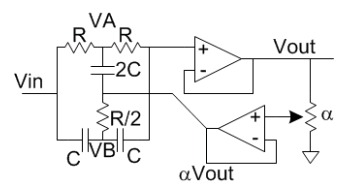
\includegraphics[scale=1]{Notch}
\end{center}
After analysis in the warmup my transfer function was: $\frac{s^2 + \frac{1}{R^2C^2}}{s^2 +\frac{4(1-\alpha)}{RC} + \frac{1}{R^2C^2}}$. With this transfer function $f0=\frac{1}{2\pi RC}$ With this information we want to eliminate the 60Hz noise so we set $f0=60$ and we are given that $C=270pF$. We solve for R and find R to be $9.82M\Omega$. Using matlab I generated the following Bode plot:
\begin{center}
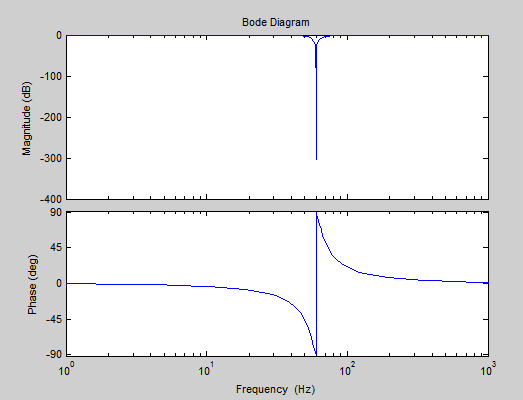
\includegraphics[scale=.75]{Notchmatlab}
\end{center}
Note the phase looks interesting because the bodeplot function probably doesn't use atan2. As we can see the bode plot dips at approximately 60 Hz. I then simulated the circuit in Multisim.\begin{center}
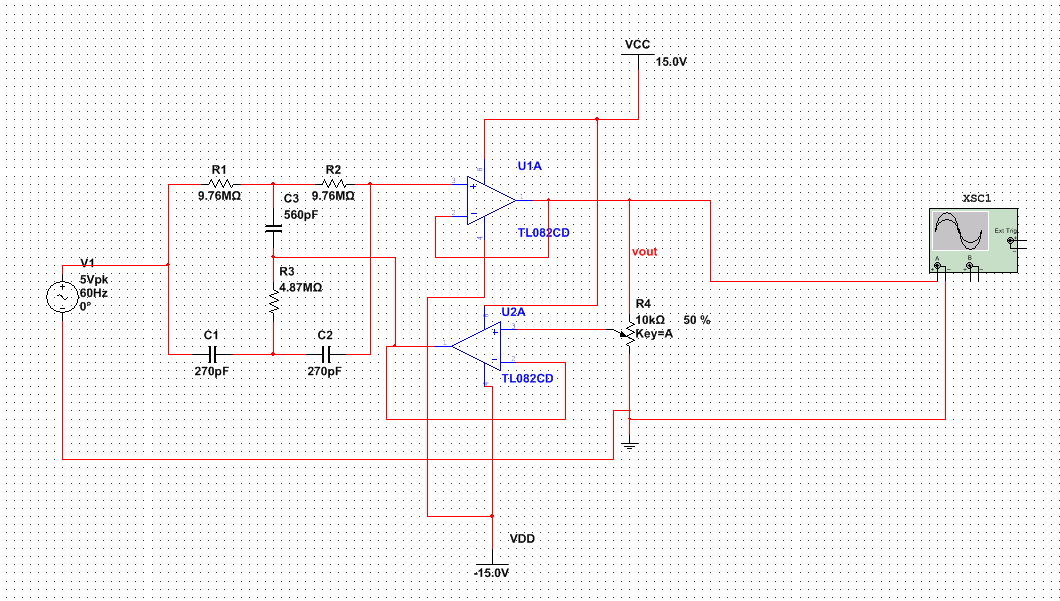
\includegraphics[scale=.5]{Circuit}
\end{center}
First I ran a montecarlo simulation:
\begin{center}
\includegraphics[scale=1]{montecarlo}
\end{center}
The filter has a dip around 60 Hz which is what we want.\\\\
I then fed 3 different AC signals into the filter 10Hz,60Hz, and 500Hz.\\
10Hz:
\begin{center}
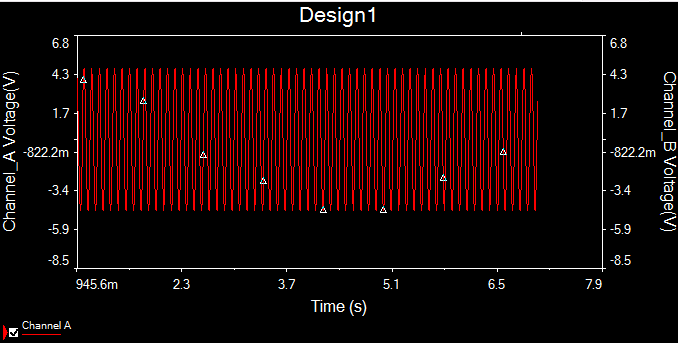
\includegraphics[scale=1]{10Hz}
\end{center}
60Hz:
\begin{center}
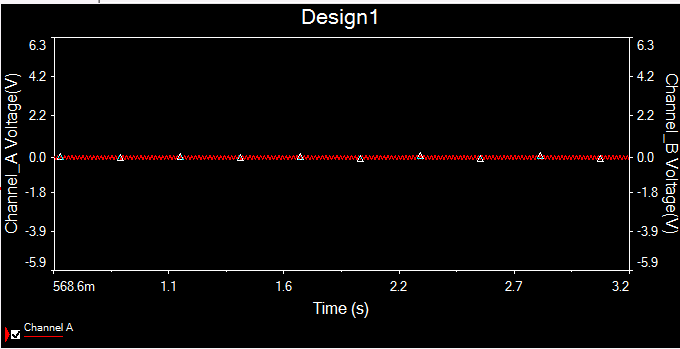
\includegraphics[scale=1]{60Hzsim}
\end{center}
500Hz:
\begin{center}
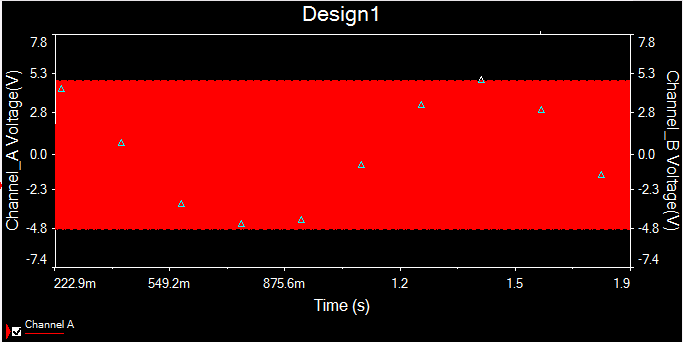
\includegraphics[scale=1]{500Hz}
\end{center}
As we can see 10Hz and 500Hz retain their amplitude while 60Hz gets cutoff.\\\\
\textbf{Sallen Keys}
For the Sallen Keys Portion I again used my transfer function from the warmup questions and got: $\frac{\frac{1}{R6*C6*C5*R5}}{s^2 + s*\frac{R6+R5}{R6*C6*R5}+\frac{1}{R6*C6*C5*R5}}$ From this we get $wn=\sqrt{\frac{1}{R6*C6*C5*R5}}$ and $\zeta = \frac{R6+R5}{2*(R6*C6*R5)}*\sqrt{R6*C6*C5*R5}$ To come up with values for the Sallen Keys filter I knew I wanted the cutoff frequency to be 140Hz and that we want the filter to decay quickly so we need a critically damped system $\zeta =1$. I set the capacitors to $0.1\mu F$ and solved for the resistors and got both resistors should be $R=11,368\Omega$. The filter looks like the following:
\begin{center}
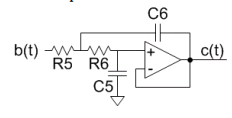
\includegraphics[scale=1]{Sallen}
\end{center}
I used matlab to generate the Bode Plot:
\begin{center}
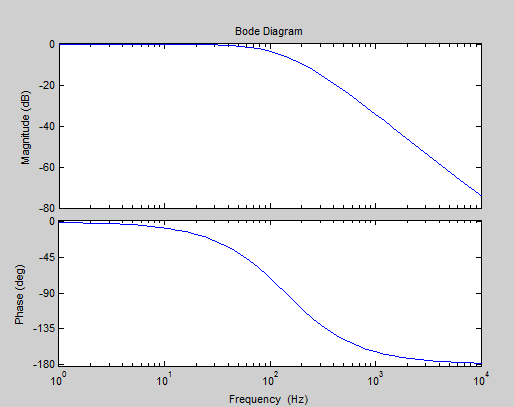
\includegraphics[scale=.75]{sallenKeys}
\end{center}
I then ran a montecarlo simulation on the full circuit:
\begin{center}
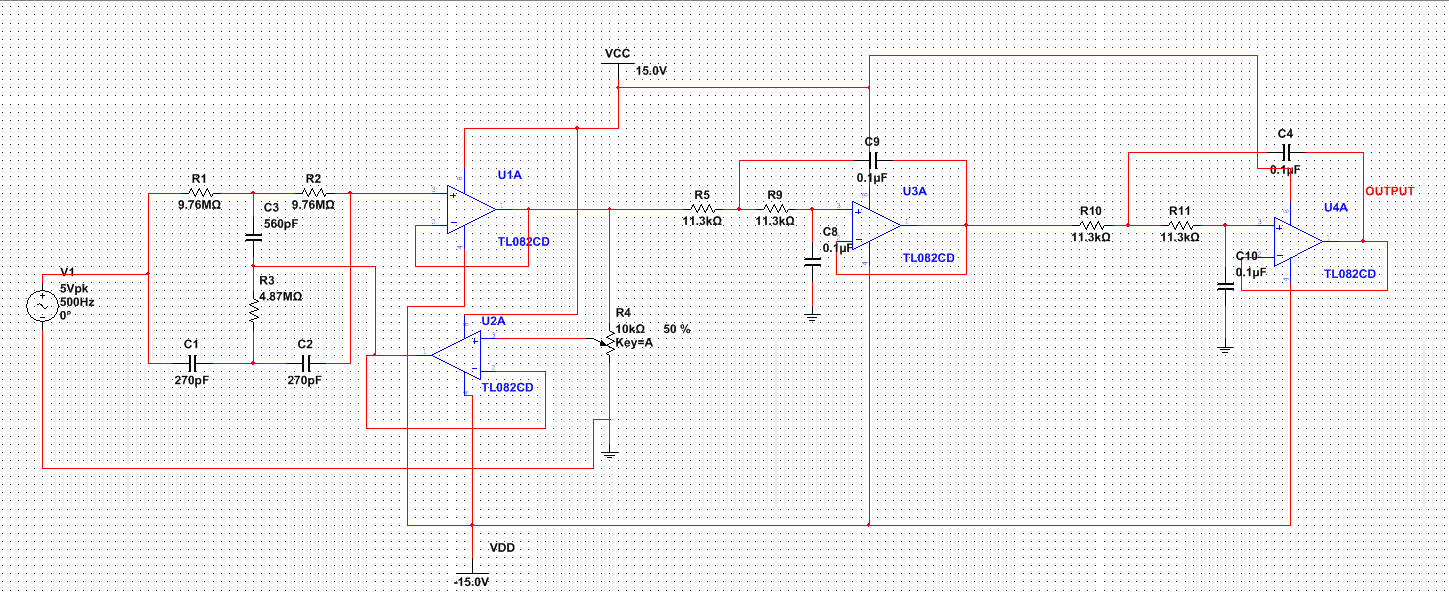
\includegraphics[scale=.5]{fullcircuit}
\end{center}
\begin{center}
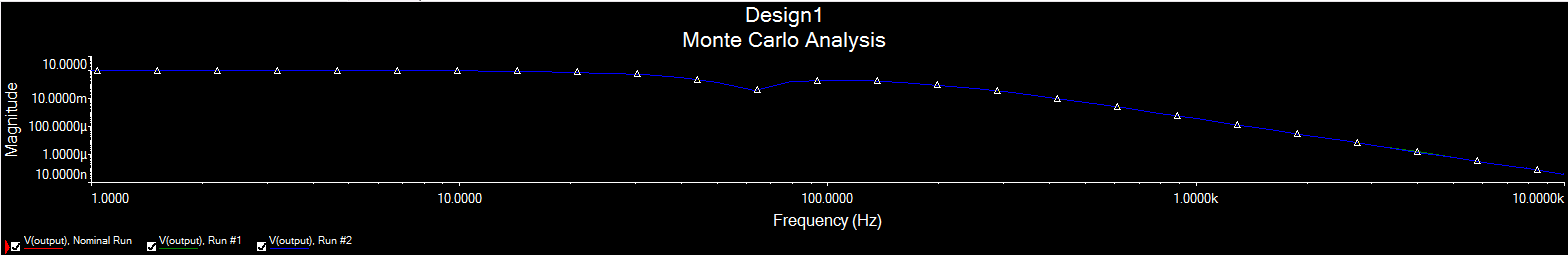
\includegraphics[scale=.5]{FullMontecarlo}
\end{center}
We have the cutoff at 60Hz as well as the dive downward at around 140 Hz from the simulation.\\\\
\textbf{Lab}
For the lab I tested my circuit on a breadboard as shown below:
\begin{center}
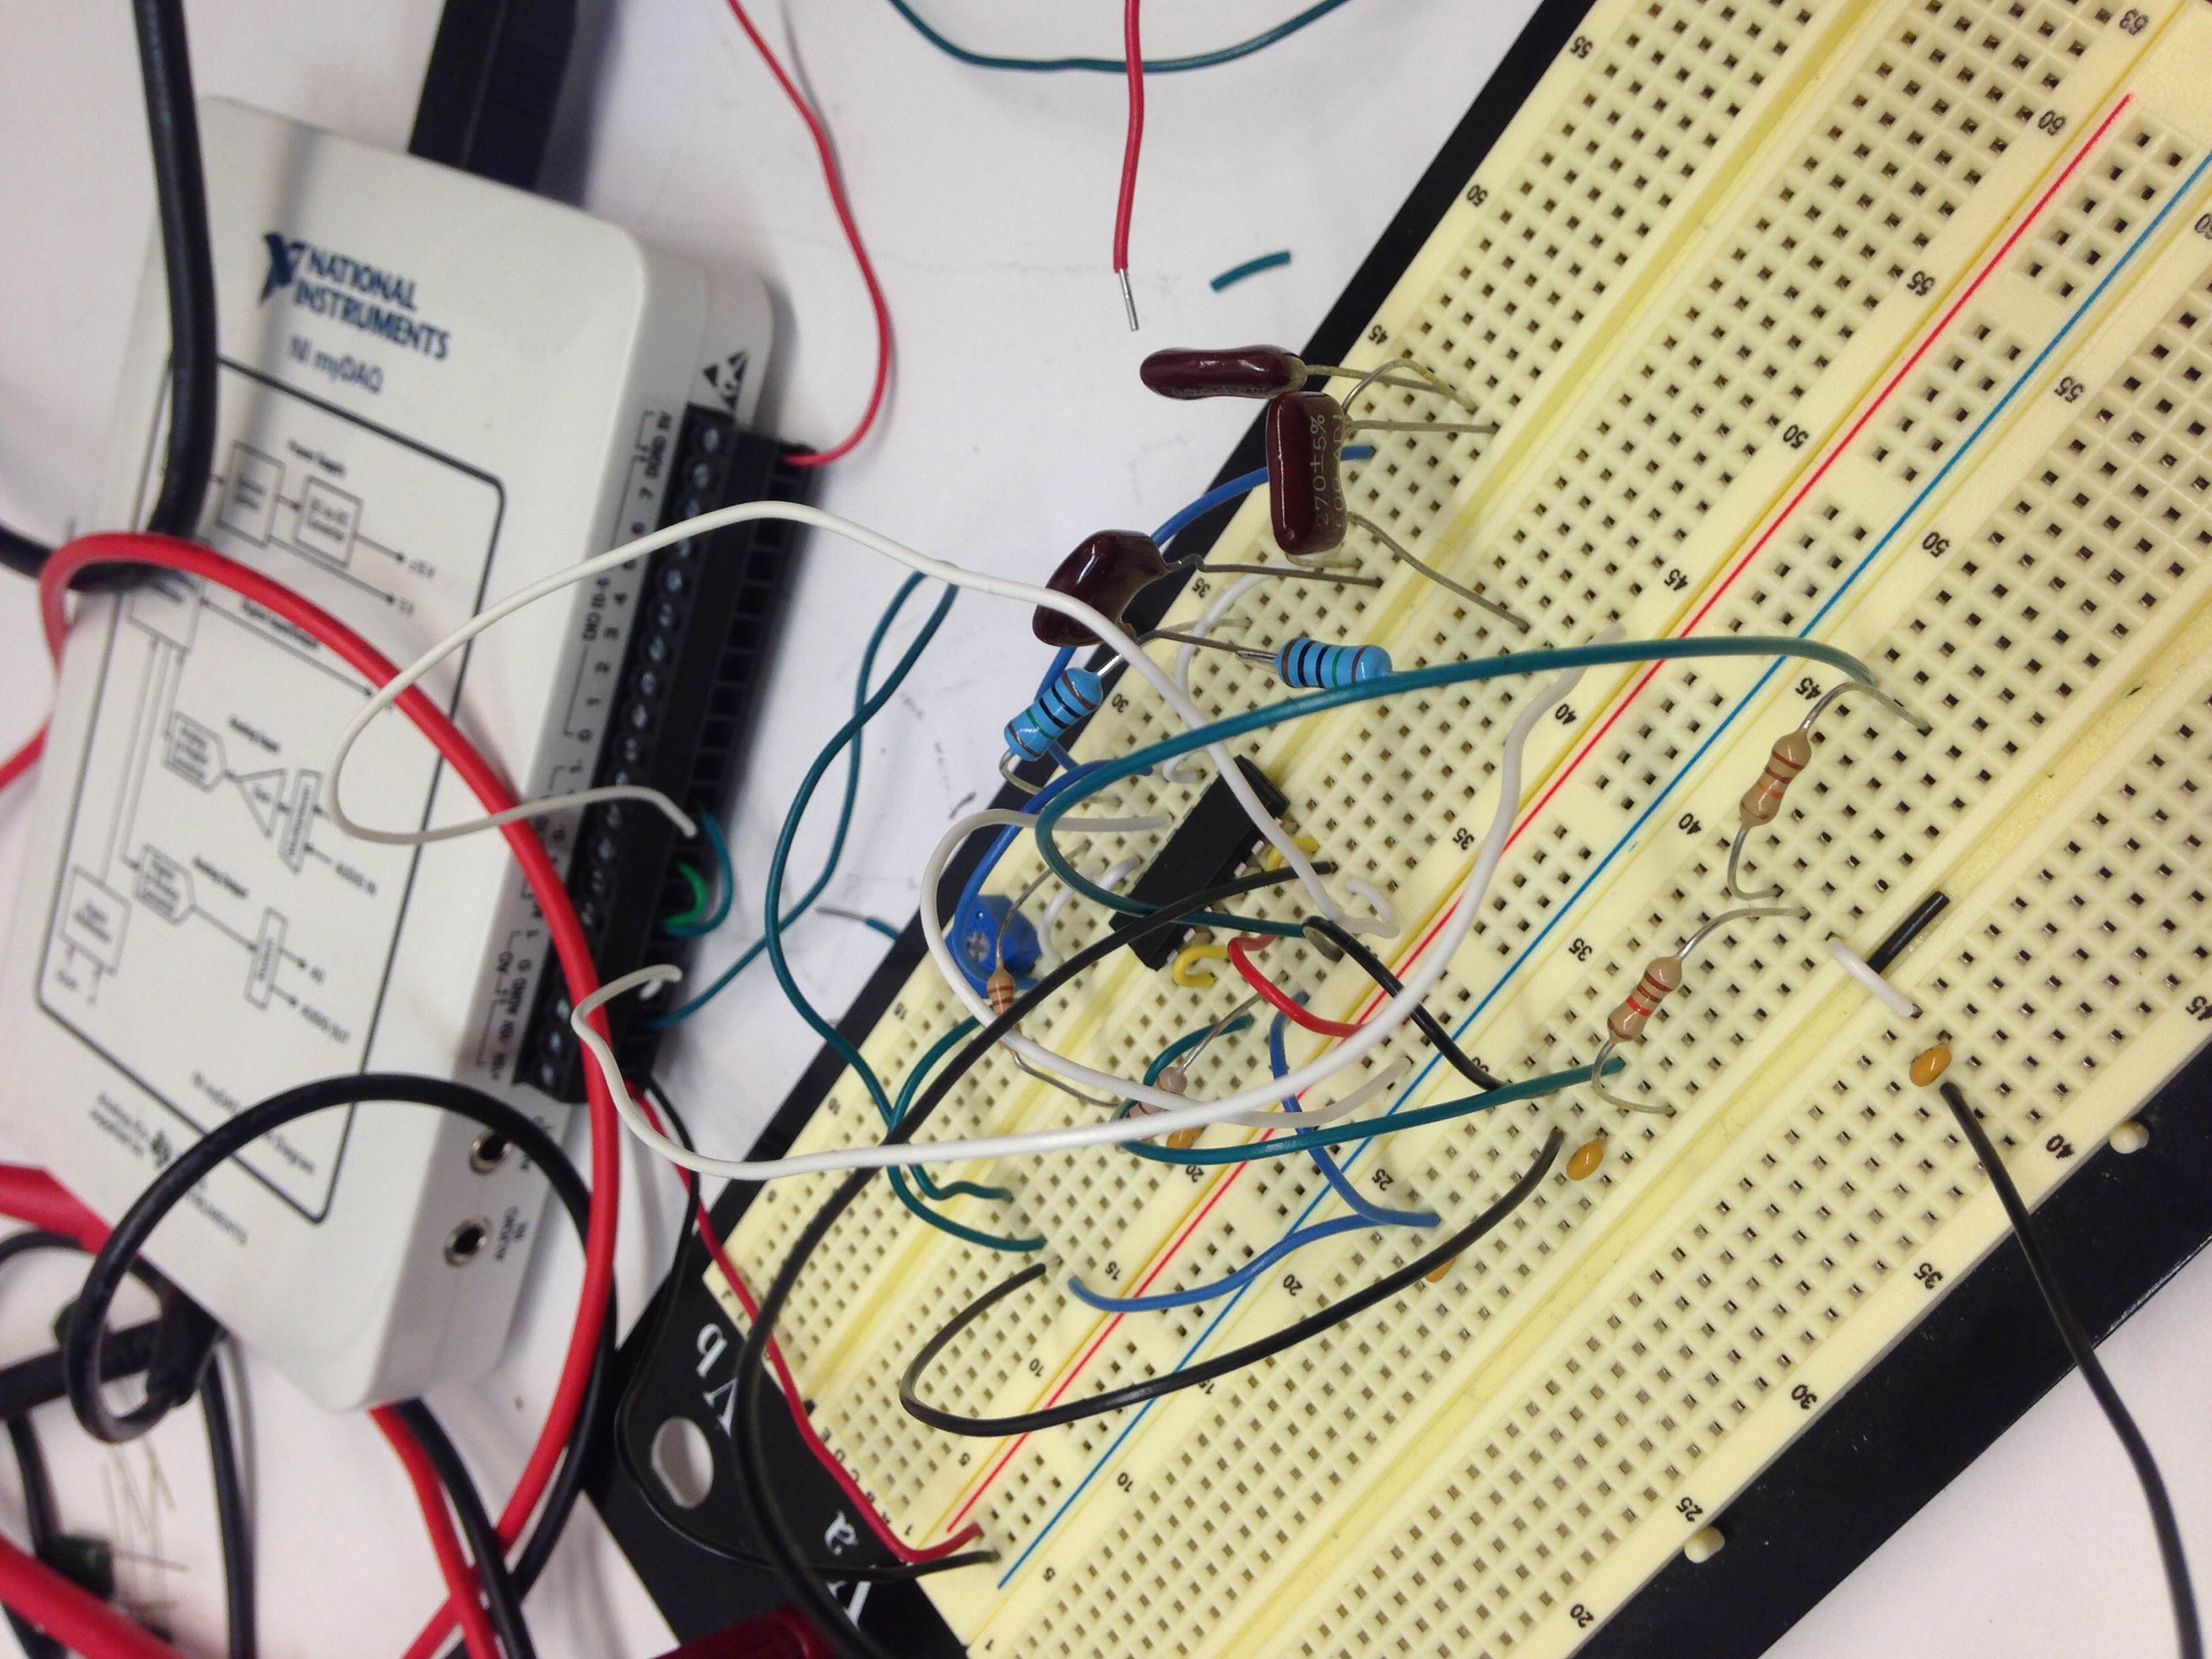
\includegraphics[scale=.1]{realcirc}
\end{center}
I tested the circuit on a number of frequencies from 20Hz to 200Hz with 20Hz intervals. Here are a few of the outputs:
\newpage
20Hz:
\begin{center}
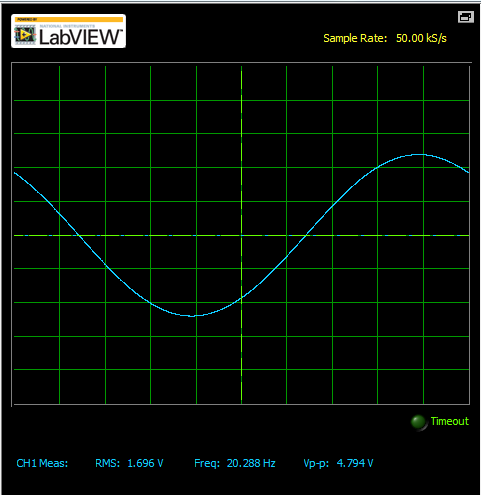
\includegraphics[scale=.8]{20Hz}
\end{center}
60Hz:
\begin{center}
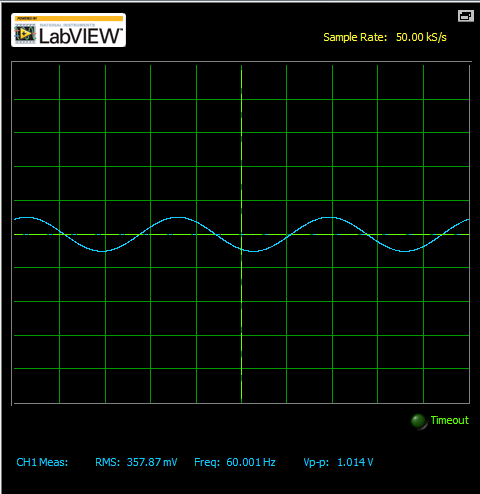
\includegraphics[scale=.8]{60Hz}
\end{center}
\newpage
100Hz:
\begin{center}
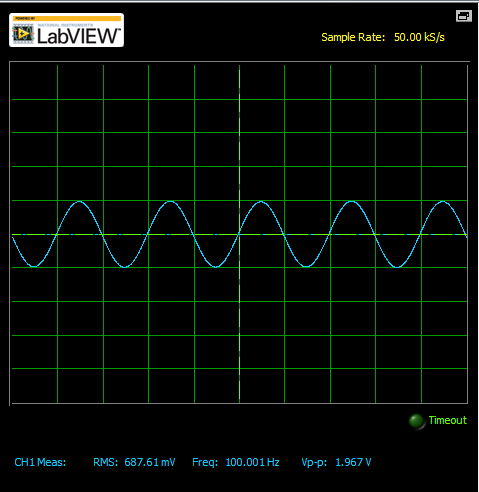
\includegraphics[scale=.8]{100Hz}
\end{center}
200Hz:
\begin{center}
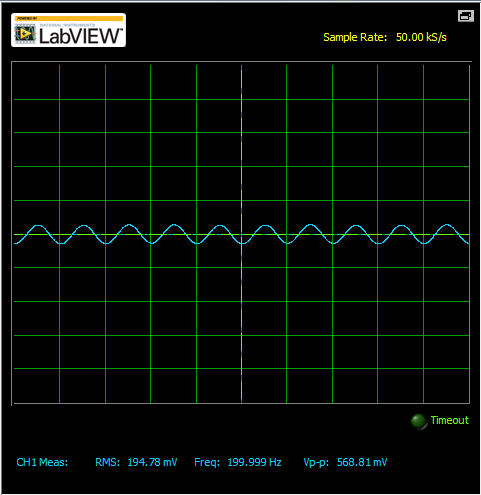
\includegraphics[scale=.8]{200Hz}
\end{center}
\newpage
1000Hz:
\begin{center}
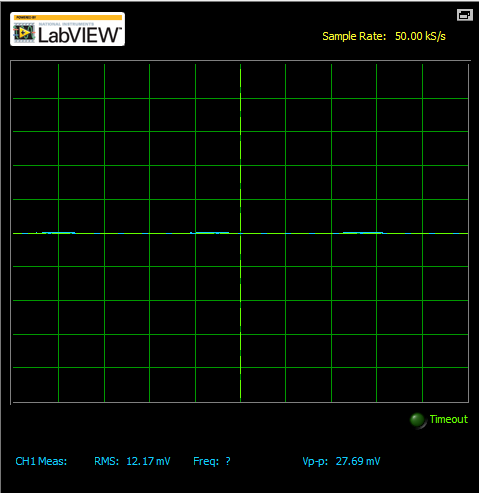
\includegraphics[scale=.8]{1000Hz}
\end{center}

From the graphs shown It appears that the filters are working the way they are supposed to. Prior to 60Hz we see little attenuation, at 60Hz we see a severe drop in magnitude. After 60Hz we see a rise in magnitude until 140Hz where we see a decline in magnitude. My plots don't show very steep cutoffs for 60Hz and 140Hz and I believe it is because I forgot to tune the potentiometer when testing my circuit, however my plots show that my circuit followed the expected behavior.




\end{document}